\begin{center}
	\LARGE
	Uden hjælpemidler
\end{center}
\begin{opgavetekst}{Opgave 1}
\end{opgavetekst}
\begin{delopgave}{1}
	Løs ligningen $\ln(x)(x^2-x-2) = 0$.
\end{delopgave}
%
%
%
%
%
%
\begin{opgavetekst}{Opgave 2}
	En trekant $\triangle ABC$ er givet på Figur \ref{fig:tangens}.
	\begin{figure}[H]
		\centering
		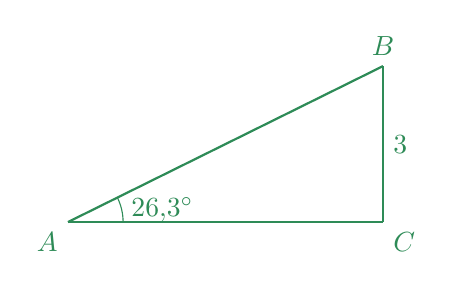
\begin{tikzpicture}
			\draw[color = SeaGreen, thick] (0,0) -- (4,0)
			node[anchor = north east, pos = 0] {$A$} 
			node[anchor = north west, pos = 1] {$C$};
			\draw[color = SeaGreen, thick] (0,0) -- (4,1.98)
			node[anchor = south, pos = 1] {$B$};
			\draw[color = SeaGreen, thick] (4,0) -- (4,1.98)
			node[anchor = west, pos = 0.5] {$3$};
			\draw[color = SeaGreen] (0.7,0) arc (0:26.3:0.7)
			node[anchor = west, pos = 0.5] {$26,\!3^\circ$};
		\end{tikzpicture}
		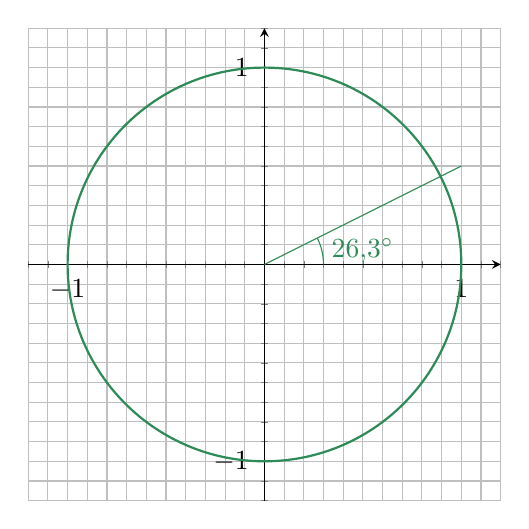
\begin{tikzpicture}
		\begin{axis}
			[
			axis lines = center, 
			xmin = -1.2, xmax = 1.2, 
			ymin = -1.2, ymax = 1.2,
			x = 2.5cm, y = 2.5cm,
			xtick = {-2,-1,...,1,2},
			ytick = {-2,-1,...,1,2},
			minor tick num = 9,
			grid = both
			]
			\draw[color = SeaGreen, thick] (axis cs: 0,0) circle (1);
			\draw[color = SeaGreen] (axis cs: 0,0) -- (axis cs: 1,0.5);
			\draw[color = SeaGreen] (axis cs: 0.3,0) arc (0:26.3:{2.5*0.3cm})
			node[pos = 0.5, anchor = west] {$26,\!3^\circ$};
		\end{axis}
		\end{tikzpicture}
		\caption{Trekanten $\triangle ABC$ samt en enhedscirkel med markeret vinkel.}
		\label{fig:tangens}
	\end{figure}
	\phantom{h}
\end{opgavetekst}
\begin{delopgave}{1}
	Bestem længden af linjestykket $b$ ved at bruge Figur 
	\ref{fig:tangens}.
\end{delopgave}
%
%
%
%
%
\begin{opgavetekst}{Opgave 3}
	En differentialligning er givet ved
	\begin{align*}
		\frac{dy}{dx} = y + x^2
	\end{align*}
\end{opgavetekst}
\begin{delopgave}{1}
	Vis, at $f(x) = -x^2 - 2x - 2 + e^x$ er en løsning til differentialligningen. 
\end{delopgave}
%
%
%
%
%
\newpage
\begin{opgavetekst}{Opgave 4}
	To linjer $l$ og $m$ er givet ved
	\begin{align*}
		&l: \ (2 + t)(x - 5) + 2(y + 12) = 0,\\
		&m: \ t(x + 1) - 4(y - 3) = 0.
	\end{align*}
\end{opgavetekst}
\begin{delopgave}{1}
	Bestem de værdier for $t$, der gør linjerne $l$ og $m$ vinkelrette. 
\end{delopgave}
%
%
%
%
%
\begin{opgavetekst}{Opgave 5}
	En linje $l$ er givet ved ligningen
	\begin{align*}
		l: \ -3x + 4y + 16 = 0. 
	\end{align*}
\end{opgavetekst}
\begin{delopgave}{1}
	Bestem afstanden mellem linjen $l$ og punktet $P(2,10)$.
\end{delopgave}
%
%
%
%
%
\begin{opgavetekst}{Opgave 6}
	På planeten Glorp er alt foruroligende tæt på at være som på Jorden. Glorperne iklæder sig dog på en lidt særpræget måde.
	De tager 2 par bukser på, tre t-shirts på og et enkelt par sokker. 
\end{opgavetekst}
\begin{delopgave}{1}
	Bestem antallet af måder, glorperen Gibulip Glop kan tage tøj på, hvis han ejer 5 par bukser, 6 t-shirts og 10 par sokker. Gibulip Glop er ligeglad med rækkefølgen, han har taget sine lag på i. 
\end{delopgave}
%
%
%
%
%

\begin{opgavetekst}{Opgave 7}
	En funktion $f$ er givet ved
	\begin{align*}
		f(x) = (2x + 1)\sin(x^2 + x + 5).
	\end{align*}
\end{opgavetekst}
\begin{delopgave}{1}
	Bestem $\int f(x) dx$.
\end{delopgave}
\newpage
%
%%%%%%%%%%%%%%%
%
%
%

\begin{center}
	\LARGE
	Med hjælpemidler
\end{center}
\begin{opgavetekst}{Opgave 8}
	En funktion $f$ er givet ved
	\begin{align*}
		f(x) = \ln(x)\cdot \sqrt{x} - \frac{1}{10}x^2, \quad x > 0.
	\end{align*}
\end{opgavetekst}
\begin{delopgave}{1}
	Tegn grafen for $f$ på intervallet $]0,8]$.
\end{delopgave}	
\begin{delopgave}{2}
	Bestem monotoniforholdene for $f$ ved at bruge $f'$. 
\end{delopgave}
%
%
%
%
%
\begin{opgavetekst}{Opgave 9}
	En cirkel $c$ er givet ved ligningen 
	\begin{align*}
		c: \ (x-3)^2 + (y-7)^2 = 36
	\end{align*}
	og en linje $l$ er givet ved parameterfremstillingen
	\begin{align*}
		l: \
		\begin{pmatrix}
			x \\ y
		\end{pmatrix} =
		\begin{pmatrix}
			2 \\ -9
		\end{pmatrix} + 
		t
		\begin{pmatrix}
			3 \\ 10
		\end{pmatrix}
	\end{align*}
\end{opgavetekst}
\begin{delopgave}{1}
	Bestem skæringspunkterne mellem $c$ og $l$.
\end{delopgave}
%
%
%
%
%
%
\begin{opgavetekst}{Opgave 10}
	En funktion $g$ er givet ved
	\begin{align*}
		g(x) = b\cdot x^a
	\end{align*}
\end{opgavetekst}
\begin{delopgave}{1}
	Bestem tallene $a$ og $b$ så $g$ opfylder, at $g(2) = 6$ og $g(5) = 15$.
\end{delopgave}
\begin{delopgave}{2}
	Løs ligningen $g(x) = 20$.
\end{delopgave}
%
%
%
%
%
\newpage
\begin{opgavetekst}{Opgave 11}
	Antallet af bakterier $B$ i en bakteriekoloni kan beskrives ved differentialligningen
	\begin{align*}
		\frac{dB}{dt} = 0.016\cdot B\cdot (155 - B),
	\end{align*}
	hvor $B$ betegner antallet af bakterier i mia. og $t$ betegner tiden i antal døgn efter begyndelsen af målingen.
\end{opgavetekst}
\begin{delopgave}{1}
	Bestem en forskrift for $B$, hvis det oplyses, at der efter $0$ døgn er 15 mia. bakterier. 
\end{delopgave}
\begin{delopgave}{2}
	Bestem væksthastigheden af bakterierne efter $2$ døgn. 
\end{delopgave}
\begin{delopgave}{3}
	Bestem det totale antal bakterier, der har været i kolonien i løbet af de første 5 døgn, hvis det oplyses, at bakterierne har en levetid på 1 døgn.
\end{delopgave}
%
%
%
%
%
\begin{opgavetekst}{Opgave 12}
	En funktion $h$ er givet ved 
	\begin{align*}
		h(x) = \sin(x)x^2 - 0.2x^3 + 2, \quad  0 \leq h \leq 2\pi,
	\end{align*}
	afgrænser sammen med koordinatakserne et område $M$.
\end{opgavetekst}	
\begin{delopgave}{1}
	Bestem arealet af $M$. 
\end{delopgave}
\begin{meretekst}
	Når $M$ roteres om $x$-aksen, danner det et omdrejningslegeme $O$.
\end{meretekst}
\begin{delopgave}{2}
	Bestem rumfanget af $O$. 
\end{delopgave}